\section{Motivations}
The analysis of animal behaviour is essential for wildlife conservation and management \parencite{Greggor2019, singh2020animal}. Researchers often utilize video cameras for action recognition to conduct long-term and consistent animal behaviour analysis. This technology enables a deeper understanding of animal populations, ecosystems, health and needs, movement-related injuries, and behavioural changes \parencite{ng2022animal, Giersberg:2022aa, 8259762}.

Due to the varying temporal scales across different animal actions, video footage allows continuous monitoring of multiple animals over different time scales \parencite{ANDERSON201418}. However, recognizing animal actions in videos is challenging since they are usually collected in the wild, capturing a wide variety of actions performed by different animal species with varying sizes, textures, shapes, and motion speeds. Despite these challenges, the majority of research has focused on human action recognition, resulting in a relatively underexplored domain of animal action recognition \parencite{mondal2023msqnet}.

Fortunately, the recent introduction of the Animal Kingdom dataset \parencite{ng2022animal} at the Computer Vision and Pattern Recognition Conference (CVPR) 2022 addresses this gap. This dataset comprises 50 hours of video clips showcasing up to 850 unique species and 140 fine-grained action classes, making it a valuable resource for animal action recognition. This dataset offers an invaluable opportunity to advance animal action recognition methodologies. This research utilizes the Animal Kingdom dataset for both model training and evaluation.

\section{Challenges}
\subsection{Long-Tail Issue}
The first challenge in animal action recognition is the long-tail issue. Since animal behaviour footage is typically collected in the wild, animal action datasets often contain imbalanced data for different actions, reflecting their natural distribution. While common actions are routinely observed, rare actions might be documented with significantly lower frequency. This makes the collection of these videos costly and leads to insufficient samples \parencite{ng2022animal, perrett2023use}. As deep learning models are data-driven, the long tail distribution has been a huge challenge for network training, which leads to poor performance on less frequent classes \parencite{cao2019learning, zhang2021videolt}.

Figure \ref{fig:1_1_LongTail} illustrates the long-tail nature of the Animal Kingdom dataset. It is evident that the dataset is highly imbalanced. The frequent classes account for 80\% of the dataset, while the less frequent and rare classes form only less than 20\%.

\begin{figure}[ht]
    \centering
    % \includegraphics[width=1.0\textwidth]{assets/charts/1_1_LongTail}
    \resizebox{1.0\textwidth}{!}{\input{"assets/charts/1_1_LongTail.pgf"}}
    \caption[Action Classes Frequency Distribution]{This Chart shows the long-tail distribution of action class frequency. On the graph, the X-axis represents the action index, and the y-axis displays the action count. The action classes in green colour are frequent classes, while the action classes in blue and red colour are less frequent or rare classes.}
    \label{fig:1_1_LongTail}
\end{figure}

\begin{figure}[ht]
    \centering
    % \includegraphics[width=1\textwidth]{assets/charts/1_2_ClassEmbeddingInternVideo}
    \adjustbox{trim=6.2cm 2cm 5cm 2cm}{%
        \resizebox{1.4\textwidth}{!}{\input{"assets/charts/1_2_ClassEmbeddingInternVideo.pgf"}}
    }
    \caption[Class Embedding Distribution]{This figure shows the distribution of class embeddings. The 140 action classes are converted into sentences using the prompt template "A video of an animal <action>. This action is a kind of <category of action> behaviour.", which is then encoded into embedding by the text encoding module of InternVideo \parencite{wang2022internvideo}. By applying Principle Component Analysis to reduce the dimension, the embeddings can be plotted in the 2D plane. Green labels represent the head classes; blue labels represent the middle classes; red labels represent the tail classes.}
    \label{fig:1_2_ClassEmbeddingInternVideo}
\end{figure}

It has been proved that the distance of text embeddings strongly correlates with semantic similarity, even allowing for meaningful arithmetic calculations \parencite{mikolov2013efficient}. As Figure \ref{fig:1_2_ClassEmbeddingInternVideo} shows, applying the principle component analysis on the text embedding generated by the InternVideo's \parencite{wang2022internvideo} video CLIP module reveals relationships between classes. For example, the movement actions such as walking, running, flying, and landing are clustered at the right-bottom of the figure, while the birth-related actions such as giving birth, laying eggs, hatching and undergoing chrysalis, are gathered at the top of the figure. 

By encoding text and visual data into the same semantic space, I am able to transfer the learning target of the model from one-hot encoding to a class embedding in the semantic space \parencite{ma2022x}, which might mitigate the unbalanced distribution caused by the long-tail issue. 


\subsection{Temporal Redundancy}
The second challenge is the temporal redundancy. Numerous animal actions exhibit subtle motions, and this high temporal redundancy can confuse the recognition model \parencite{YUAN2018221, li2022uniformer}. Figure \ref{fig:1_3_FrameComparison} illustrates this redundancy. 

\begin{figure}[ht]
    \centering
    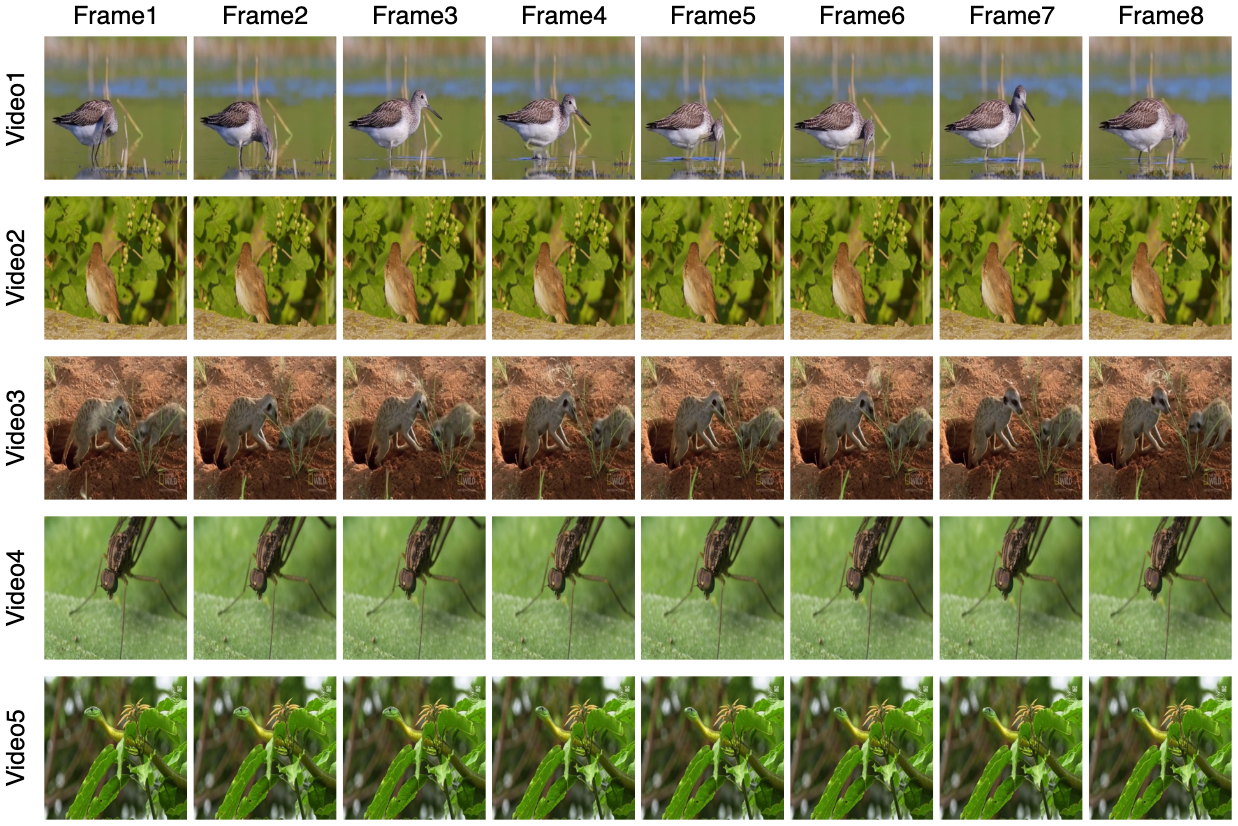
\includegraphics[width=1\textwidth]{assets/charts/1_3_FrameComparison}
    \caption[Temporal Redundancy]{This figure illustrates the high temporal redundancy between neighbouring frames in animal videos. Each row of the figure shows sampled frames from the same video.}
    \label{fig:1_3_FrameComparison}
\end{figure}

To enhance the capability to capture fine-grained texture differences between neighbouring frames, this research introduces the Action Frame Contrastive Learning Network (AFRICAN). This network functions as a counterpart to Contrastive Language-Image Pre-training (CLIP) \parencite{radford2021learning} focusing more on semantic meaning. It forces the model to extract fine-grained feature differences between similar frames in the same video. 

% TODO: may be updated after picking the epoch for score table
\section{Contributions}
In this research, two primary contributions are presented. Firstly, CLIP model is demonstrated to be able to effectively tackle the long-tail issue in animal action recognition, improving 21.9\% and 20.7\% mAP on middle and tail classes, while improving only 6.2\% mAP on head classes. Secondly, the AFRICAN network can serve as an auxiliary enhancer, aiding the model in understanding the temporal dimension of animal actions, improving the around 1\% mAP to achieve 55.08\% mAP.

